\documentclass{article}

\usepackage[final]{../neurips_2019}

\usepackage[utf8]{inputenc}
\usepackage[T1]{fontenc}
\usepackage{hyperref}
\usepackage{url}
\usepackage{booktabs}
\usepackage{amsfonts}
\usepackage{amsmath, bm, bbm}
\usepackage{amssymb}
\usepackage{nicefrac}
\usepackage{microtype}
\usepackage{graphicx}
\usepackage{xcolor}
\usepackage{lipsum}
\usepackage{makecell}

\newcommand{\note}[1]{\textcolor{blue}{{#1}}}

\title{
  Exploring CNNs in Question Answering \\
  \vspace{1em}
  \small{\normalfont Stanford CS224N Default Project}  % Select one and delete the other
}

\author{
  Joseph Pagadora, $\;$ Steve Gan \\
  Stanford University \\
  \texttt{jcp737@stanford.edu}$\;\;\;\;$
  \texttt{zgan@stanford.edu} \\
  % Examples of more authors
%   \And
%   Name \\
%   Department of Computer Science \\
%   Stanford University \\
%   \texttt{name@stanford.edu} \\
%   \And
%   Name \\
%   Department of Computer Science \\
%   Stanford University \\
%   \texttt{name@stanford.edu}
}

\begin{document}

\maketitle

% \begin{abstract}
%   Required for final report
% \end{abstract}

\begin{abstract}
The goal of this project is to reproduce the QANet model described in [??] and improve on this model. So far, we have focused on an implementation of QANet in PyTorch. < <--\texttt{Sentence on experimental results}--> >. As explained in the proposal, for the rest of the project we plan to also implement the data augmentation approach through backtranslation, and furthermore, we plan to explore improvement ideas such as span representation and tweaking the attention mechanism and the backtranslation pipeline.
\end{abstract}

\section{Approach}
\subsection{Model}
The SQuAD dataset is a standard dataset used for the NLP task of question-answering. At a basic level, a datapoint in SQuAD consists of a triple $(C, Q, S),$ where $C$ is the context paragraph, $Q$ is a question, and $S$ is a span in the context $C$ that contains the answer to the question $Q.$
\begin{figure}[h]
\centering
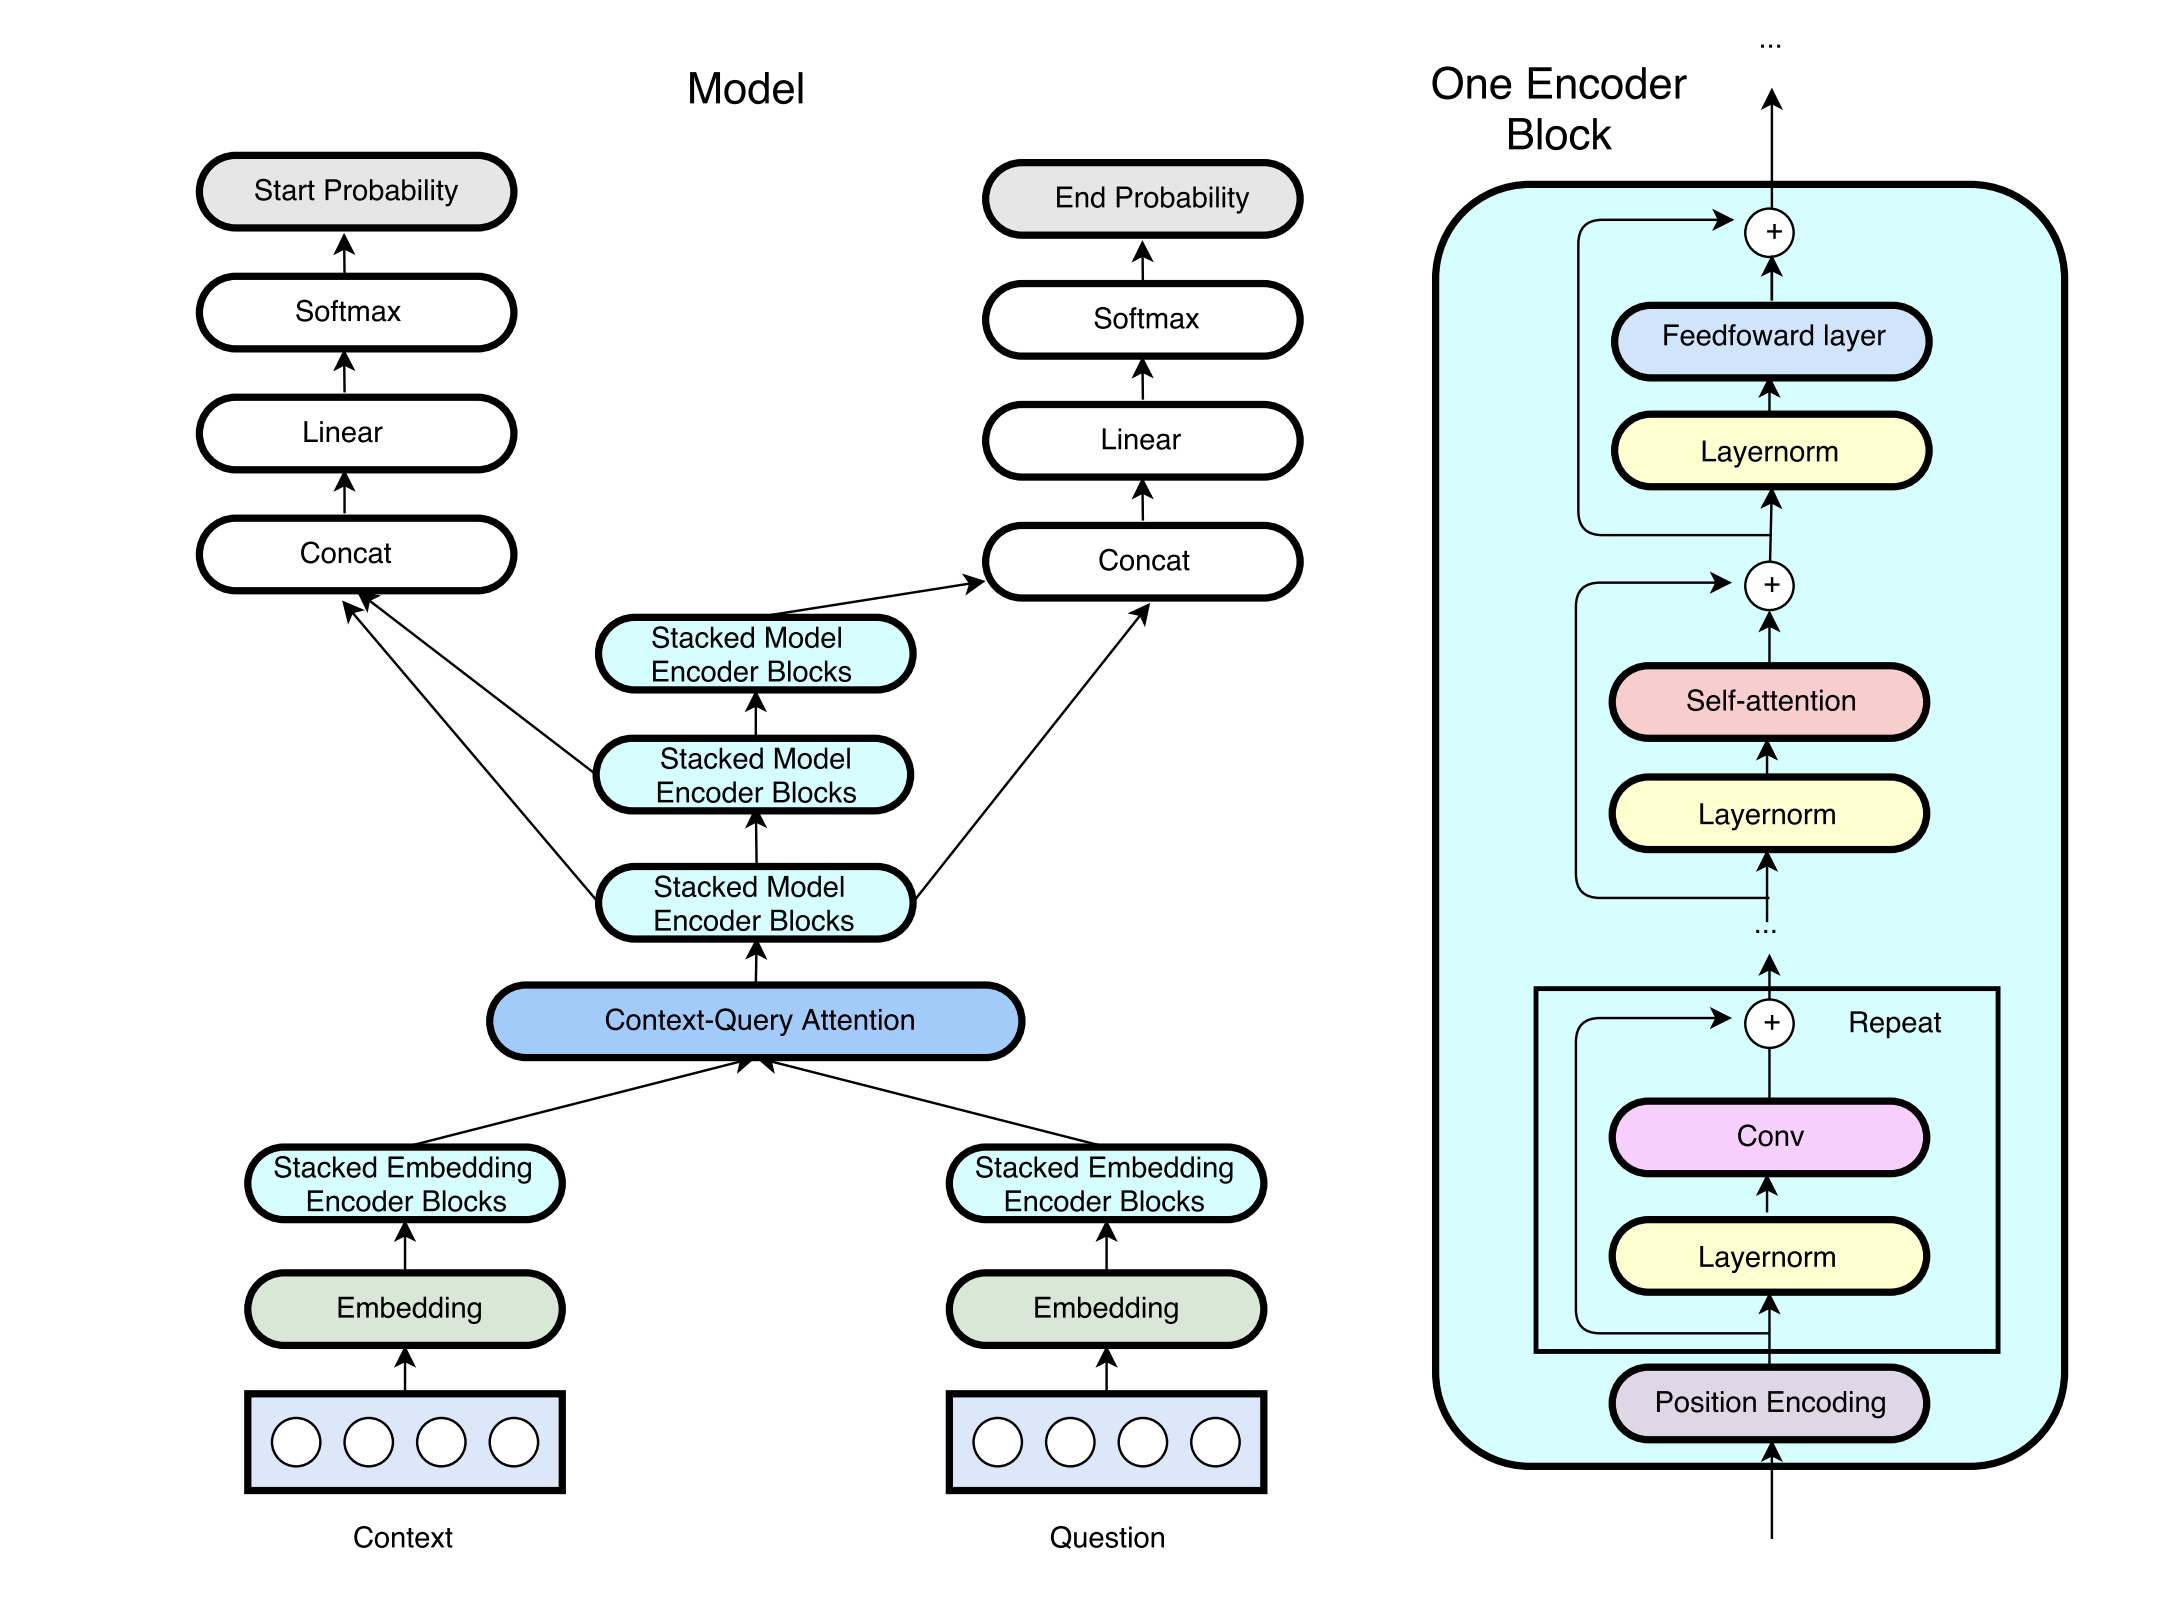
\includegraphics[scale=0.23]{../model_diagram}
\caption{Left: Architecture of QANet with convolution and self-attention. Right: Encoder block that is used throughout the model.}
\end{figure}
We implemented a version of the QANet model, which is summarized in Figure 1. Words are embedded using (1) GLoVE (300-dimensional), and (2) max-pooling of character embeddings (200-dimensional). In (2), words are truncated/padded to be length 16. These two resulting embeddings are concatenated to form a 500-dimensional embedding for each word. This is done separately for context words and question words. \\
The main block for this model is the Encoder Block, each consisting of a position-encoding [??], followed by at least one 1-dimensional convolutional layer, followed by a self-attention layer, and finally a feedforward layer. Each of these, except the position-encoding, is immediately preceded by a layer-norm operation, all inside a residual block, to allow for training a deep architecture [??]. \\
After the initial embeddings of context and question words, we send each through one encoder block with 4 convolutional layers. The outputs of these are then sent to a context-query attention layer, which is a standard technique similarly done in BiDAF [??], so we refer to the method there. \\
Following this are three model encoder blocks which are in sequential order, i.e., share weights. Each consists of 7 encoder blocks with 2 convolutional layers. The output layer calculates, for each word in the context, the probabilities that (1) it is the start, or (2) the end, of the answer-containing span. This is done by computing 
$$p_{\text{start}}(i)=\text{softmax}(W_1[M_0;M_1]),\;\;\;\; p_{\text{end}}(i)=\text{softmax}(W_2[M_0;M_2]),$$
where $M_0,M_1,$ and $M_2$ denote the outputs of these blocks respectively, $[\cdot \;; \cdot]$ denotes concatenation, and $W_1,W_2$ are trainable parameters.

\subsection{Baseline}
For now, we mainly compare the performance of our initial QANet implementation with the performance of a basic BiDAF model, whose implementation was given.

\section{Experiments}
\subsection{Data}
We will use the default SQuAD dataset and the specified preprocessing methods.

\subsection{Evaluation}
We will use standard exact-match (EM) and F1 scores. The exact-match score only counts outputs that are exact matches to the labeled span, while the F1 score is less stringent by calculating the harmonic mean of the precision and recall of the outputs against the labeled span.

\subsection{Experimental Details}

\subsection{Results}

\section{Future Work}
For future work, we will use the backtranslation data-augmentation technique described in the QANet paper in order to significantly increase the size of our training set.

\bibliographystyle{unsrt.bst}
\bibliography{references}

\end{document}












